%=====================================================================
% Modelo de datos · Tablas de la fase posterior
%   Lo generado sale de bd/fase_posterior/crear_tablas_fase_posterior.sql
%   con bd/generar_tablas.ps1 (-Prefijo bdFp) y de er/generar.py.
%=====================================================================
\subsection*{Tablas de la fase posterior}
\addcontentsline{toc}{subsection}{Tablas de la fase posterior}

Estas \bdFpNumTablas{} tablas, con \bdFpNumColumnas{} atributos y \bdFpNumForaneas{} llaves foráneas, solo las escriben casos de uso marcados como fase posterior (\mbox{D-22}). No se crean con el núcleo: las crea \at{bd/fase\_posterior/crear\_tablas\_fase\_posterior.sql}, que se ejecuta sobre una base que ya tiene el núcleo y que además agrega a \textit{Usuario}, \textit{EstadisticaModo}, \textit{Partida}, \textit{Jugada} y \textit{Sala} las columnas de la subsección \textit{Revisión del esquema}. Se documentan completas para que la fase posterior empiece desde un diseño ya revisado. \bdFpNumFNBC{} de ellas cumplen la forma normal de Boyce-Codd; \textit{Equipamiento} y \textit{ParticipacionObjeto} se quedan en tercera forma normal por el motivo que explica la verificación de la normalización.

\subsubsection*{Entidades}
\addcontentsline{toc}{subsubsection}{Entidades de la fase posterior}
% Archivo generado por bd/generar_tablas.ps1 a partir de bd/fase_posterior/crear_tablas_fase_posterior.sql. No editar a mano.
\begin{center}\small
\begin{longtable}{|L{0.24\textwidth}|L{0.17\textwidth}|L{0.49\textwidth}|}
\hline
\textbf{Entidad} & \textbf{Clase} & \textbf{Qué representa} \\ \hline
\endfirsthead
\hline
\textbf{Entidad} & \textbf{Clase} & \textbf{Qué representa} \\ \hline
\endhead
\multicolumn{3}{|l|}{\textbf{Catálogos precargados de la fase posterior (\mbox{D-09})}} \\ \hline
\textit{Ranura} & Catálogo & Catálogo de las seis ranuras de personalización: peón, muro, tablero, título, marco y emotes (\mbox{D-03}). \\ \hline
\textit{Objeto\-Cosmetico} & Catálogo & Catálogo de objetos cosméticos. Cada objeto pertenece a una sola ranura (\mbox{D-03}). \\ \hline
\textit{Division} & Catálogo & Catálogo de divisiones del ranking con sus umbrales de ascenso y descenso. \\ \hline
\textit{Nivel\-IA} & Catálogo & Catálogo de los cuatro niveles de la IA (\mbox{DES-09} \mbox{RN-02}). \\ \hline
\textit{Leccion} & Catálogo & Catálogo de las siete lecciones del tutorial (\mbox{DES-16} \mbox{RN-01}). \\ \hline
\textit{Tipo\-Caja} & Catálogo & Catálogo de tipos de caja que se venden o se otorgan (\mbox{DES-14}). \\ \hline
\textit{Tipo\-Caja\-Objeto} & Catálogo asociativo & Objetos que puede contener cada tipo de caja y su probabilidad; es la relación N:M entre TipoCaja y ObjetoCosmetico. \\ \hline
\multicolumn{3}{|l|}{\textbf{Perfil y personalización}} \\ \hline
\textit{Historial\-Nickname} & Dependiente (1:0..1) & Cambio de nombre de una cuenta, para que un jugador reportado no se vuelva irreconocible (\mbox{DES-06} \mbox{RN-03}). Se borra al dar de baja la cuenta (\mbox{DES-05}). \\ \hline
\textit{Avatar} & Fuerte & Imagen subida por el jugador como foto de perfil (\mbox{CU-07} \mbox{FA-01}). \\ \hline
\textit{Enlace\-Red} & Fuerte & Enlace a una red social que el jugador muestra en su perfil (\mbox{CU-07}). \\ \hline
\textit{Usuario\-Objeto} & Asociativa (N:M) & Objetos cosméticos que posee cada cuenta; es la relación N:M entre Usuario y ObjetoCosmetico (relación Posee del diagrama). \\ \hline
\textit{Equipamiento} & Asociativa (N:M) & Objeto que cada cuenta lleva equipado en cada ranura; siempre hay exactamente uno por ranura (\mbox{DES-07} \mbox{RN-01}). \\ \hline
\multicolumn{3}{|l|}{\textbf{Aspecto en partida y espectador}} \\ \hline
\textit{Participacion\-Objeto} & Asociativa (N:M) & Aspecto con el que cada jugador entró a la partida, una fila por ranura; no cambia aunque el jugador equipe otra cosa (\mbox{DES-07} \mbox{RN-03}, \mbox{DES-12} \mbox{RN-03}). \\ \hline
\textit{Enlace\-Espectador} & Fuerte & Enlace compartido para ver una partida desde fuera del juego. Es lo único que se guarda de los espectadores (\mbox{D-19}). \\ \hline
\multicolumn{3}{|l|}{\textbf{Invitaciones}} \\ \hline
\textit{Invitacion} & Fuerte & Invitación a jugar, que da acceso a una sala sin conocer su código (\mbox{CU-23}). \\ \hline
\multicolumn{3}{|l|}{\textbf{Clasificación y economía}} \\ \hline
\textit{Historial\-Division} & Fuerte & Cambio de división de una cuenta en un modo. No se deduce de una sola partida por las partidas de margen, así que se guarda (\mbox{DES-08}). \\ \hline
\textit{Caja} & Fuerte & Caja comprada u obtenida al subir de nivel. Existe sin abrir entre la compra y la apertura (\mbox{DES-14} \mbox{RN-09}). \\ \hline
\textit{Caja\-Contenido} & Débil & Los tres objetos que salieron al abrir una caja, registrados para poder comprobarlos después (\mbox{DES-14} \mbox{RN-07}). \\ \hline
\textit{Movimiento\-Moneda} & Fuerte & Entrada o salida de monedas. El saldo verdadero es su suma; nunca se modifica ni se elimina (\mbox{DES-15} \mbox{RN-01}). \\ \hline
\multicolumn{3}{|l|}{\textbf{Relaciones entre jugadores y tutorial}} \\ \hline
\textit{Amistad} & Asociativa (N:M) & Amistad recíproca entre dos cuentas, guardada una sola vez por par ordenado (\mbox{CU-22} \mbox{RN-03}). \\ \hline
\textit{Solicitud} & Fuerte & Solicitud de amistad pendiente. Tiene dirección, a diferencia de la amistad, y se borra al responderse (\mbox{CU-21}, \mbox{CU-22}). \\ \hline
\textit{Progreso\-Tutorial} & Asociativa (N:M) & Avance de cada cuenta en cada lección del tutorial; es la relación N:M entre Usuario y Leccion (\mbox{DES-16}). \\ \hline
\end{longtable}
\end{center}


\subsubsection*{Diagramas}
\addcontentsline{toc}{subsubsection}{Diagramas de la fase posterior}
Uno por área. Las entidades del núcleo que sus relaciones tocan, como \textit{Usuario} o \textit{Participacion}, aparecen sin atributos.

\begin{center}
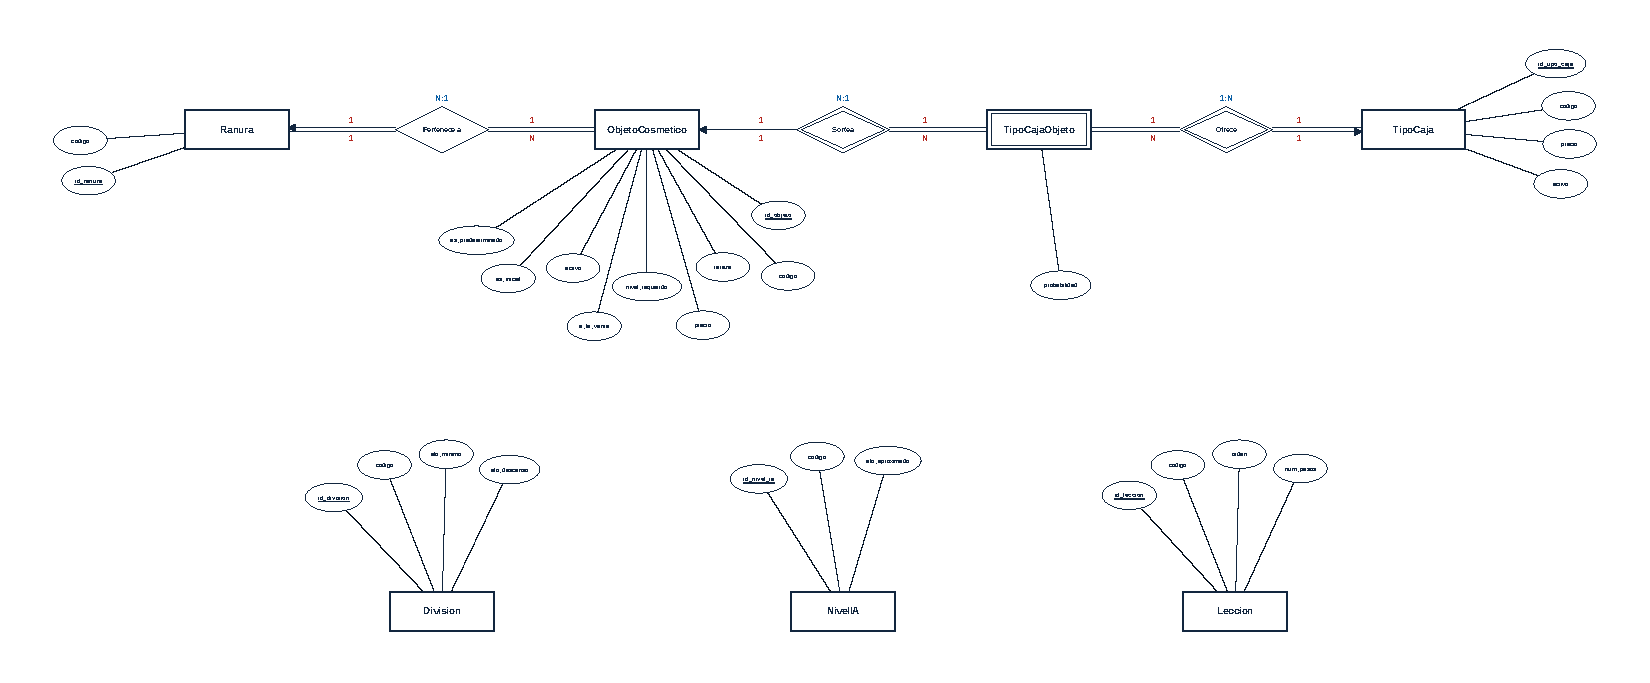
\includegraphics[width=\linewidth,height=0.42\textheight,keepaspectratio]{er/salida/fp-catalogos}\par\smallskip
{\small Catálogos de la fase posterior.}
\end{center}
\begin{center}
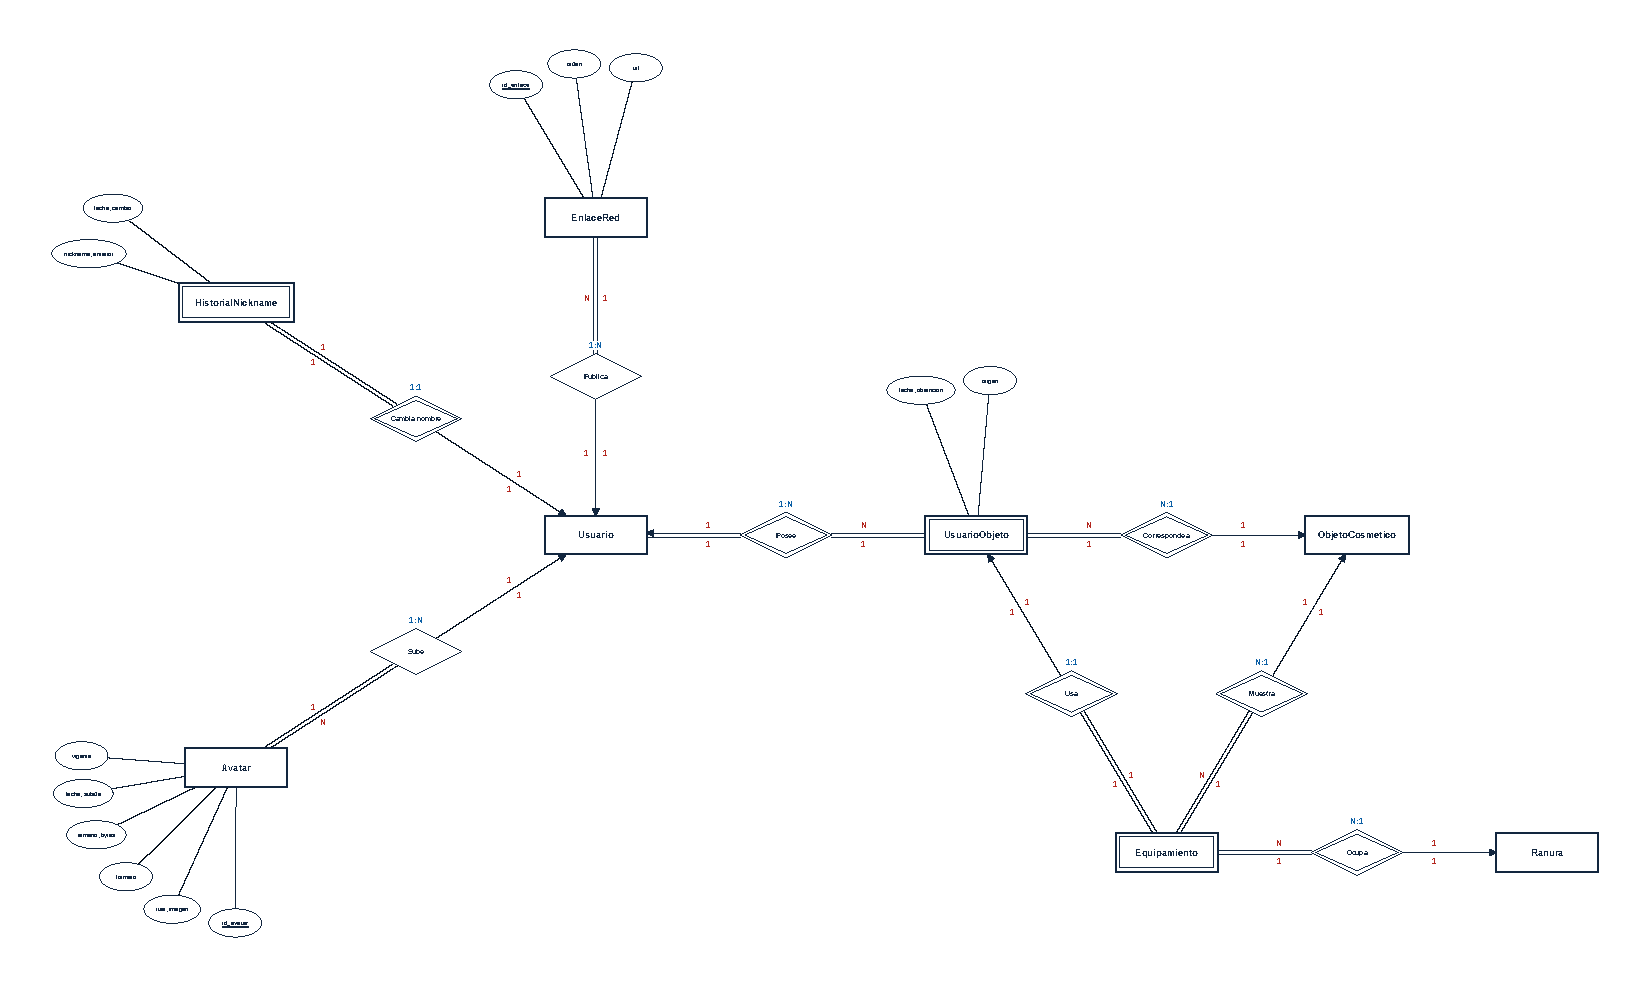
\includegraphics[width=\linewidth,height=0.42\textheight,keepaspectratio]{er/salida/fp-perfil}\par\smallskip
{\small Perfil y personalización.}
\end{center}
\begin{center}
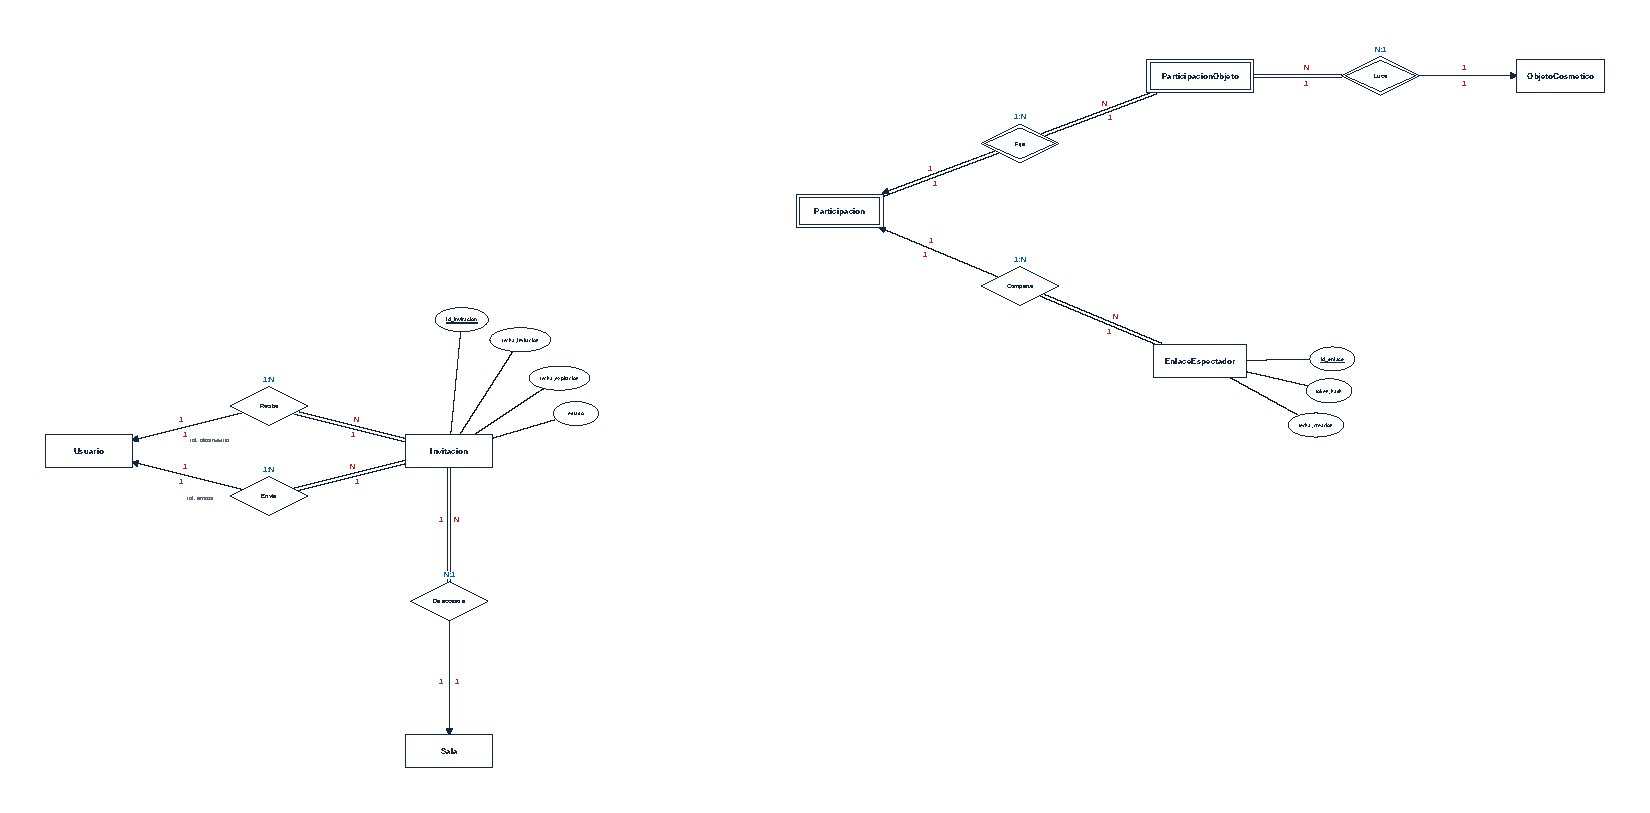
\includegraphics[width=\linewidth,height=0.42\textheight,keepaspectratio]{er/salida/fp-partida}\par\smallskip
{\small Aspecto en partida, espectador e invitaciones.}
\end{center}
\begin{center}
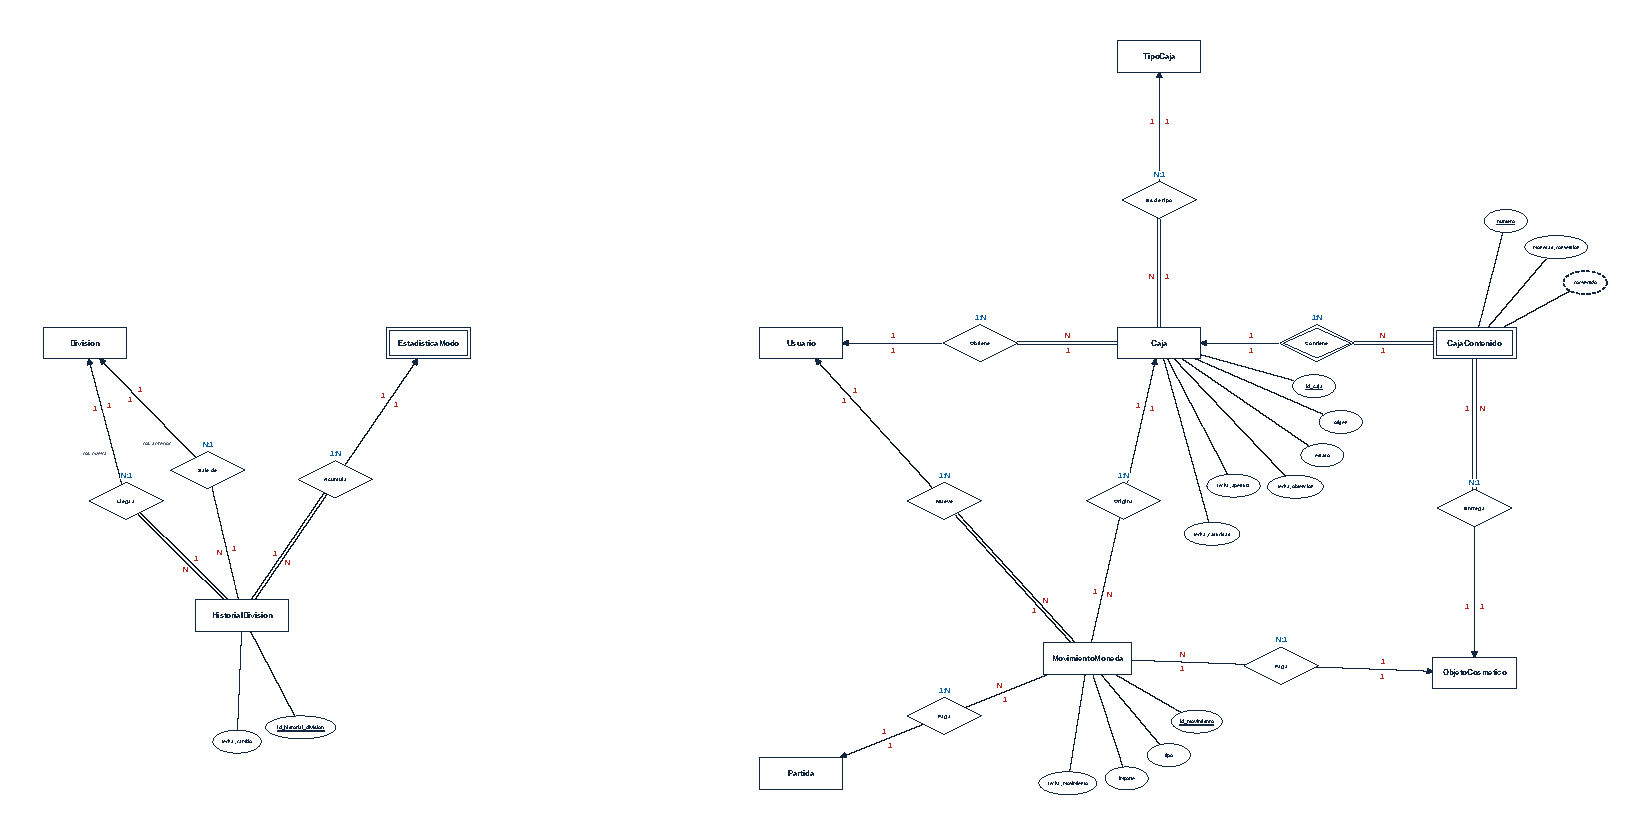
\includegraphics[width=\linewidth,height=0.42\textheight,keepaspectratio]{er/salida/fp-economia}\par\smallskip
{\small Clasificación y economía.}
\end{center}
\begin{center}
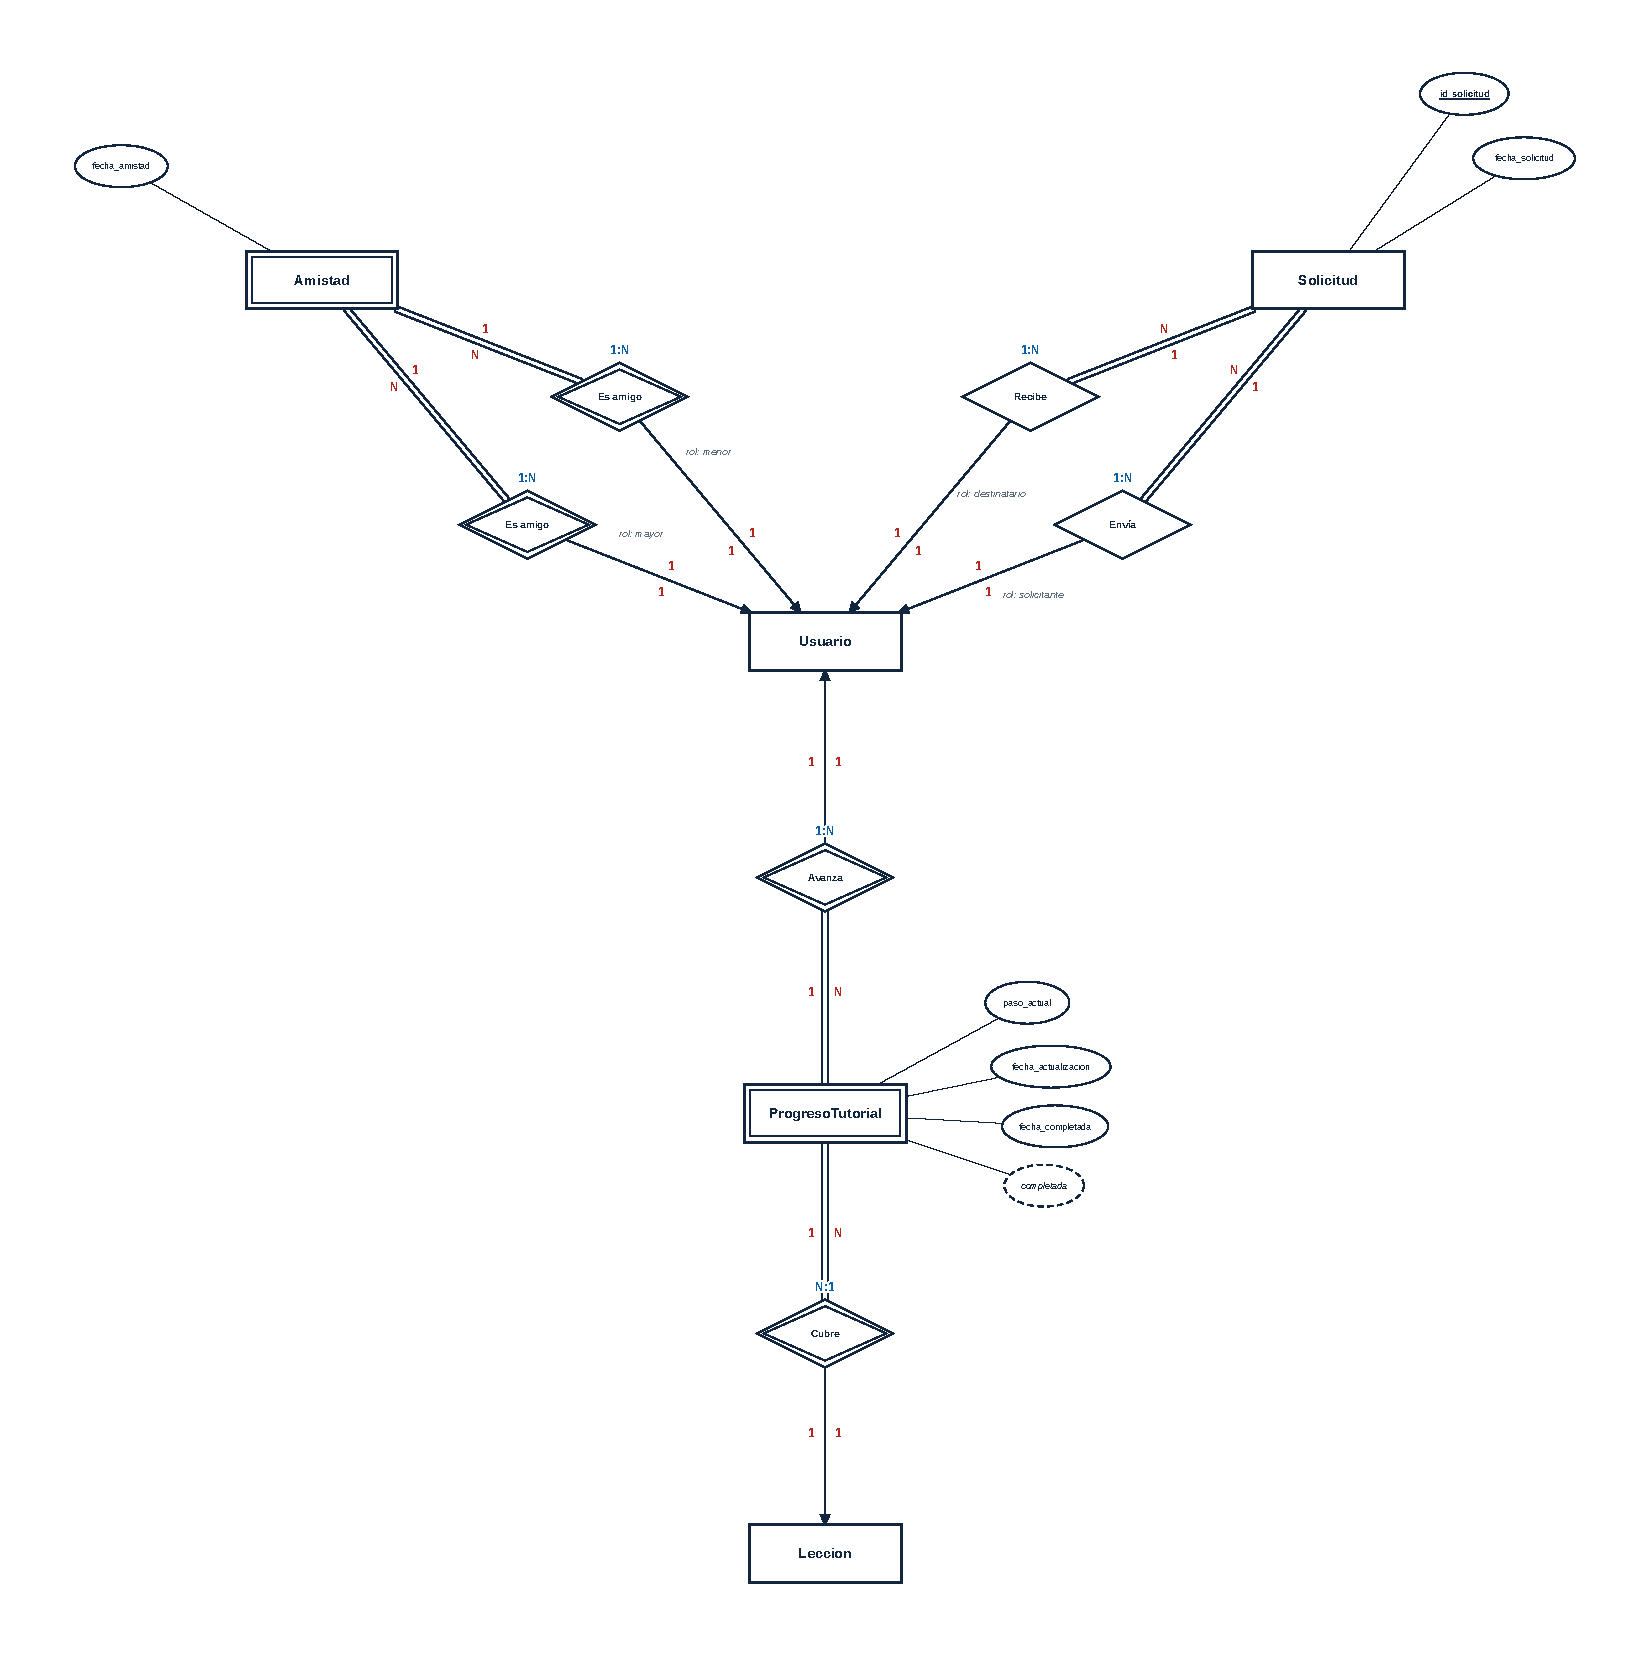
\includegraphics[width=\linewidth,height=0.42\textheight,keepaspectratio]{er/salida/fp-social}\par\smallskip
{\small Relaciones entre jugadores y tutorial.}
\end{center}

\subsubsection*{Atributos}
\addcontentsline{toc}{subsubsection}{Atributos de la fase posterior}
% Archivo generado por bd/generar_tablas.ps1 a partir de bd/fase_posterior/crear_tablas_fase_posterior.sql. No editar a mano.
% Archivo generado por bd/generar_tablas.ps1 a partir de bd/fase_posterior/crear_tablas_fase_posterior.sql. No editar a mano.
\subsubsection*{
Catálogos precargados de la fase posterior (\mbox{D-09})
}
\addcontentsline{toc}{subsubsection}{
Catálogos precargados de la fase posterior (\mbox{D-09})
}

\atributosde{Ranura}{Catálogo de las seis ranuras de personalización: peón, muro, tablero, título, marco y emotes (\mbox{D-03}).}
\begin{tablaatributos}
\texttt{id\_\allowbreak{}ranura} & \texttt{TINYINT} & No & PK & Identificador de la ranura. \\ \hline
\texttt{codigo} & \texttt{VARCHAR(20)} & No & UQ & Clave de la ranura en los diccionarios de recursos (\mbox{D-21}): \texttt{PEON}, \texttt{MURO}, \texttt{TABLERO}, \texttt{TITULO}, \texttt{MARCO} o \texttt{EMOTES}. Sin CHECK: añadir una ranura es insertar una fila (\mbox{CU-14}). \\ \hline
\end{tablaatributos}

\atributosde{ObjetoCosmetico}{Catálogo de objetos cosméticos. Cada objeto pertenece a una sola ranura (\mbox{D-03}).}
\begin{tablaatributos}
\texttt{id\_\allowbreak{}objeto} & \texttt{INT} & No & PK & Identificador del objeto. \\ \hline
\texttt{id\_\allowbreak{}ranura} & \texttt{TINYINT} & No & FK & Ranura en la que se equipa. \\ \hline
\texttt{codigo} & \texttt{VARCHAR(40)} & No & UQ & Clave del objeto en los diccionarios de recursos, como \texttt{PEON\_\allowbreak{}CLASICO}; con ella el cliente muestra su nombre en el idioma del usuario (\mbox{D-21}). \\ \hline
\texttt{rareza} & \texttt{VARCHAR(10)} & No &  & \texttt{COMUN}, \texttt{RARO}, \texttt{EPICO} o \texttt{LEGENDARIO}. \\ \hline
\texttt{precio} & \texttt{INT} & No &  & Precio en monedas del juego; el válido es este y no el del cliente (\mbox{CU-38} \mbox{RN-03}). Por omisión, \texttt{0}. \\ \hline
\texttt{nivel\_\allowbreak{}requerido} & \texttt{SMALLINT} & No &  & Nivel mínimo para comprarlo (\mbox{CU-38} \mbox{RN-04}). Por omisión, \texttt{1}. \\ \hline
\texttt{a\_\allowbreak{}la\_\allowbreak{}venta} & \texttt{BIT} & No &  & Si se ofrece en la tienda. Por omisión, \texttt{0}. \\ \hline
\texttt{activo} & \texttt{BIT} & No &  & En falso, retirado del catálogo; quien lo tiene equipado lo conserva (\mbox{CU-14} \mbox{RN-04}). Por omisión, \texttt{1}. \\ \hline
\texttt{es\_\allowbreak{}inicial} & \texttt{BIT} & No &  & Se otorga al dar de alta la cuenta. Por omisión, \texttt{0}. \\ \hline
\texttt{es\_\allowbreak{}predeterminado} & \texttt{BIT} & No &  & Se equipa al dar de alta; exactamente uno por ranura. Por omisión, \texttt{0}. \\ \hline
\end{tablaatributos}

\atributosde{Division}{Catálogo de divisiones del ranking con sus umbrales de ascenso y descenso.}
\begin{tablaatributos}
\texttt{id\_\allowbreak{}division} & \texttt{TINYINT} & No & PK & Identificador de la división. \\ \hline
\texttt{codigo} & \texttt{VARCHAR(40)} & No & UQ & Clave de la división en los diccionarios de recursos (\mbox{D-21}), como \texttt{BRONCE} o \texttt{MURO\_\allowbreak{}PIEDRA}. \\ \hline
\texttt{elo\_\allowbreak{}minimo} & \texttt{SMALLINT} & No & UQ & Elo con el que se asciende a esta división; ordena las divisiones de la más baja a la más alta. \\ \hline
\texttt{elo\_\allowbreak{}descenso} & \texttt{SMALLINT} & No &  & Elo por debajo del cual se desciende; es el umbral visible (\mbox{CU-25} \mbox{RN-07}). \\ \hline
\end{tablaatributos}

\atributosde{NivelIA}{Catálogo de los cuatro niveles de la IA (\mbox{CU-27} \mbox{RN-02}).}
\begin{tablaatributos}
\texttt{id\_\allowbreak{}nivel\_\allowbreak{}ia} & \texttt{TINYINT} & No & PK & Identificador del nivel. \\ \hline
\texttt{codigo} & \texttt{VARCHAR(40)} & No & UQ & Clave del nivel en los diccionarios de recursos (\mbox{D-21}): \texttt{APRENDIZ}, \texttt{CONSTRUCTOR}, \texttt{ARQUITECTO} o \texttt{BASTION}. \\ \hline
\texttt{elo\_\allowbreak{}aproximado} & \texttt{SMALLINT} & No &  & Fuerza aproximada: 1000, 1500, 1900 o 2300. \\ \hline
\end{tablaatributos}

\atributosde{Leccion}{Catálogo de las siete lecciones del tutorial (\mbox{CU-41} \mbox{RN-01}).}
\begin{tablaatributos}
\texttt{id\_\allowbreak{}leccion} & \texttt{TINYINT} & No & PK & Identificador de la lección. \\ \hline
\texttt{codigo} & \texttt{VARCHAR(40)} & No & UQ & Clave de la lección en los diccionarios de recursos (\mbox{D-21}), como \texttt{MOVER\_\allowbreak{}PEON}; los textos de sus pasos también están en ellos. \\ \hline
\texttt{orden} & \texttt{TINYINT} & No & UQ & Posición en el índice del tutorial. \\ \hline
\texttt{num\_\allowbreak{}pasos} & \texttt{TINYINT} & No &  & Pasos de la lección. \\ \hline
\end{tablaatributos}

\atributosde{TipoCaja}{Catálogo de tipos de caja que se venden o se otorgan (\mbox{CU-39}).}
\begin{tablaatributos}
\texttt{id\_\allowbreak{}tipo\_\allowbreak{}caja} & \texttt{TINYINT} & No & PK & Identificador del tipo de caja. \\ \hline
\texttt{codigo} & \texttt{VARCHAR(40)} & No & UQ & Clave del tipo de caja en los diccionarios de recursos (\mbox{D-21}), como \texttt{CAJA\_\allowbreak{}MADERA}. \\ \hline
\texttt{precio} & \texttt{INT} & No &  & Precio en monedas del juego. \\ \hline
\texttt{activo} & \texttt{BIT} & No &  & En falso, ya no se vende. Por omisión, \texttt{1}. \\ \hline
\end{tablaatributos}

\atributosde{TipoCajaObjeto}{Objetos que puede contener cada tipo de caja y su probabilidad; es la relación N:M entre TipoCaja y ObjetoCosmetico.}
\begin{tablaatributos}
\texttt{id\_\allowbreak{}tipo\_\allowbreak{}caja} & \texttt{TINYINT} & No & PK, FK & Tipo de caja. \\ \hline
\texttt{id\_\allowbreak{}objeto} & \texttt{INT} & No & PK, FK & Objeto que puede salir. \\ \hline
\texttt{probabilidad} & \texttt{DECIMAL(6,3)} & No &  & Porcentaje exacto que se muestra antes de comprar (\mbox{CU-39} \mbox{RN-01}). \\ \hline
\end{tablaatributos}


% Archivo generado por bd/generar_tablas.ps1 a partir de bd/fase_posterior/crear_tablas_fase_posterior.sql. No editar a mano.
\subsubsection*{
Perfil y personalización
}
\addcontentsline{toc}{subsubsection}{
Perfil y personalización
}

\atributosde{HistorialNickname}{Cambio de nombre de una cuenta, para que un jugador reportado no se vuelva irreconocible (\mbox{DES-06} \mbox{RN-03}). Se borra al dar de baja la cuenta (\mbox{DES-05}).}
\begin{tablaatributos}
\texttt{id\_\allowbreak{}usuario} & \texttt{INT} & No & PK, FK & Cuenta que cambió su nombre. Como llave primaria, impide un segundo cambio (\mbox{DES-06} \mbox{RN-01}). \\ \hline
\texttt{nickname\_\allowbreak{}anterior} & \texttt{NVARCHAR(30)} & No &  & Nombre antes del cambio. \\ \hline
\texttt{fecha\_\allowbreak{}cambio} & \texttt{DATETIME2(0)} & No &  & Momento del cambio. Por omisión, la fecha actual. \\ \hline
\end{tablaatributos}

\atributosde{Avatar}{Imagen subida por el jugador como foto de perfil (\mbox{CU-07} \mbox{FA-01}).}
\begin{tablaatributos}
\texttt{id\_\allowbreak{}avatar} & \texttt{INT}, identidad & No & PK & Identificador del avatar. \\ \hline
\texttt{id\_\allowbreak{}usuario} & \texttt{INT} & No & FK & Cuenta que lo subió. \\ \hline
\texttt{ruta\_\allowbreak{}imagen} & \texttt{NVARCHAR(260)} & No &  & Ubicación del archivo en el almacenamiento del servidor. \\ \hline
\texttt{formato} & \texttt{VARCHAR(4)} & No &  & \texttt{JPG} o \texttt{PNG} (\mbox{CU-07} \mbox{RN-05}). \\ \hline
\texttt{tamano\_\allowbreak{}bytes} & \texttt{INT} & No &  & Tamaño del archivo; hasta dos megabytes. \\ \hline
\texttt{fecha\_\allowbreak{}subida} & \texttt{DATETIME2(0)} & No &  & Momento de la subida. Por omisión, la fecha actual. \\ \hline
\texttt{vigente} & \texttt{BIT} & No &  & Si es el avatar que se muestra; el anterior pasa a falso (\mbox{CU-07} \mbox{RN-06}). Por omisión, \texttt{1}. \\ \hline
\end{tablaatributos}

\atributosde{EnlaceRed}{Enlace a una red social que el jugador muestra en su perfil (\mbox{CU-07}).}
\begin{tablaatributos}
\texttt{id\_\allowbreak{}enlace} & \texttt{INT}, identidad & No & PK & Identificador del enlace. \\ \hline
\texttt{id\_\allowbreak{}usuario} & \texttt{INT} & No & FK & Cuenta que lo publica. \\ \hline
\texttt{orden} & \texttt{TINYINT} & No &  & Posición en el perfil, de 1 a 4. \\ \hline
\texttt{url} & \texttt{NVARCHAR(500)} & No &  & Dirección web; no se admiten acortadores (\mbox{CU-07} \mbox{RN-03}). \\ \hline
\end{tablaatributos}

\atributosde{UsuarioObjeto}{Objetos cosméticos que posee cada cuenta; es la relación N:M entre Usuario y ObjetoCosmetico (relación Posee del diagrama).}
\begin{tablaatributos}
\texttt{id\_\allowbreak{}usuario} & \texttt{INT} & No & PK, FK & Cuenta que posee el objeto. \\ \hline
\texttt{id\_\allowbreak{}objeto} & \texttt{INT} & No & PK, FK & Objeto poseído. \\ \hline
\texttt{fecha\_\allowbreak{}obtencion} & \texttt{DATETIME2(0)} & No &  & Momento en que se obtuvo. Por omisión, la fecha actual. \\ \hline
\texttt{origen} & \texttt{VARCHAR(10)} & No &  & \texttt{INICIAL}, \texttt{COMPRA}, \texttt{CAJA} o \texttt{NIVEL}. \\ \hline
\end{tablaatributos}

\atributosde{Equipamiento}{Objeto que cada cuenta lleva equipado en cada ranura; siempre hay exactamente uno por ranura (\mbox{DES-07} \mbox{RN-01}).}
\begin{tablaatributos}
\texttt{id\_\allowbreak{}usuario} & \texttt{INT} & No & PK, FK & Cuenta. \\ \hline
\texttt{id\_\allowbreak{}ranura} & \texttt{TINYINT} & No & PK, FK & Ranura; con la cuenta forma la llave, así que no puede haber dos objetos en la misma ranura. \\ \hline
\texttt{id\_\allowbreak{}objeto} & \texttt{INT} & No & FK & Objeto equipado; debe ser de la ranura y debe poseerse. \\ \hline
\end{tablaatributos}


% Archivo generado por bd/generar_tablas.ps1 a partir de bd/fase_posterior/crear_tablas_fase_posterior.sql. No editar a mano.
\subsubsection*{
Aspecto en partida y espectador
}
\addcontentsline{toc}{subsubsection}{
Aspecto en partida y espectador
}

\atributosde{ParticipacionObjeto}{Aspecto con el que cada jugador entró a la partida, una fila por ranura; no cambia aunque el jugador equipe otra cosa (\mbox{DES-07} \mbox{RN-03}, \mbox{DES-12} \mbox{RN-03}).}
\begin{tablaatributos}
\texttt{id\_\allowbreak{}partida} & \texttt{INT} & No & PK, FK & Partida. \\ \hline
\texttt{id\_\allowbreak{}usuario} & \texttt{INT} & No & PK, FK & Jugador. \\ \hline
\texttt{id\_\allowbreak{}ranura} & \texttt{TINYINT} & No & PK, FK & Ranura. \\ \hline
\texttt{id\_\allowbreak{}objeto} & \texttt{INT} & No & FK & Objeto que tenía equipado en esa ranura al empezar. \\ \hline
\end{tablaatributos}

\atributosde{EnlaceEspectador}{Enlace compartido para ver una partida desde fuera del juego. Es lo único que se guarda de los espectadores (\mbox{D-19}).}
\begin{tablaatributos}
\texttt{id\_\allowbreak{}enlace} & \texttt{INT}, identidad & No & PK & Identificador del enlace. \\ \hline
\texttt{id\_\allowbreak{}partida} & \texttt{INT} & No & FK & Partida que se comparte; el enlace deja de valer cuando termina. \\ \hline
\texttt{id\_\allowbreak{}creador} & \texttt{INT} & No & FK & Participante que lo compartió. \\ \hline
\texttt{token\_\allowbreak{}hash} & \texttt{VARBINARY(32)} & No & UQ & Resumen del token del enlace. \\ \hline
\texttt{fecha\_\allowbreak{}creacion} & \texttt{DATETIME2(0)} & No &  & Momento en que se compartió. Por omisión, la fecha actual. \\ \hline
\end{tablaatributos}


% Archivo generado por bd/generar_tablas.ps1 a partir de bd/fase_posterior/crear_tablas_fase_posterior.sql. No editar a mano.
\subsubsection*{
Invitaciones
}
\addcontentsline{toc}{subsubsection}{
Invitaciones
}

\atributosde{Invitacion}{Invitación a jugar, que da acceso a una sala sin conocer su código (\mbox{CU-23}).}
\begin{tablaatributos}
\texttt{id\_\allowbreak{}invitacion} & \texttt{INT}, identidad & No & PK & Identificador de la invitación. \\ \hline
\texttt{id\_\allowbreak{}sala} & \texttt{INT} & No & FK & Sala a la que se invita. \\ \hline
\texttt{id\_\allowbreak{}emisor} & \texttt{INT} & No & FK & Jugador que invita. \\ \hline
\texttt{id\_\allowbreak{}destinatario} & \texttt{INT} & No & FK & Jugador invitado. \\ \hline
\texttt{fecha\_\allowbreak{}invitacion} & \texttt{DATETIME2(0)} & No &  & Envío. Por omisión, la fecha actual. \\ \hline
\texttt{fecha\_\allowbreak{}expiracion} & \texttt{DATETIME2(0)} & No &  & Sesenta segundos después del envío (\mbox{CU-23} \mbox{RN-03}). \\ \hline
\texttt{estado} & \texttt{VARCHAR(10)} & No &  & \texttt{PENDIENTE}, \texttt{ACEPTADA}, \texttt{RECHAZADA} o \texttt{EXPIRADA}. Por omisión, \texttt{PENDIENTE}. \\ \hline
\end{tablaatributos}


% Archivo generado por bd/generar_tablas.ps1 a partir de bd/fase_posterior/crear_tablas_fase_posterior.sql. No editar a mano.
\subsubsection*{
Clasificación y economía
}
\addcontentsline{toc}{subsubsection}{
Clasificación y economía
}

\atributosde{HistorialDivision}{Cambio de división de una cuenta en un modo. No se deduce de una sola partida por las partidas de margen, así que se guarda (\mbox{DES-08}).}
\begin{tablaatributos}
\texttt{id\_\allowbreak{}historial\_\allowbreak{}division} & \texttt{INT}, identidad & No & PK & Identificador del cambio. \\ \hline
\texttt{id\_\allowbreak{}usuario} & \texttt{INT} & No & FK & Cuenta. \\ \hline
\texttt{id\_\allowbreak{}modo} & \texttt{TINYINT} & No & FK & Modo en que cambió de división. \\ \hline
\texttt{id\_\allowbreak{}division\_\allowbreak{}anterior} & \texttt{TINYINT} & Sí & FK & División de la que sale; nula al obtener la primera. \\ \hline
\texttt{id\_\allowbreak{}division\_\allowbreak{}nueva} & \texttt{TINYINT} & No & FK & División a la que llega. \\ \hline
\texttt{fecha\_\allowbreak{}cambio} & \texttt{DATETIME2(0)} & No &  & Momento del cambio; lo marca la gráfica de elo. Por omisión, la fecha actual. \\ \hline
\end{tablaatributos}

\atributosde{Caja}{Caja comprada u obtenida al subir de nivel. Existe sin abrir entre la compra y la apertura (\mbox{DES-14} \mbox{RN-09}).}
\begin{tablaatributos}
\texttt{id\_\allowbreak{}caja} & \texttt{INT}, identidad & No & PK & Identificador de la caja. \\ \hline
\texttt{id\_\allowbreak{}usuario} & \texttt{INT} & No & FK & Cuenta dueña de la caja. \\ \hline
\texttt{id\_\allowbreak{}tipo\_\allowbreak{}caja} & \texttt{TINYINT} & No & FK & Tipo, que fija el contenido posible. \\ \hline
\texttt{origen} & \texttt{VARCHAR(10)} & No &  & \texttt{COMPRA} o \texttt{PARTIDA}. \\ \hline
\texttt{estado} & \texttt{VARCHAR(10)} & No &  & \texttt{SIN\_\allowbreak{}ABRIR}, \texttt{ABIERTA} o \texttt{CADUCADA}. Por omisión, \texttt{SIN\_\allowbreak{}ABRIR}. \\ \hline
\texttt{fecha\_\allowbreak{}obtencion} & \texttt{DATETIME2(0)} & No &  & Momento en que se obtuvo. Por omisión, la fecha actual. \\ \hline
\texttt{fecha\_\allowbreak{}apertura} & \texttt{DATETIME2(0)} & Sí &  & Momento en que se abrió. \\ \hline
\texttt{fecha\_\allowbreak{}caducidad} & \texttt{DATETIME2(0)} & Sí &  & Solo en cajas ganadas jugando, a los catorce días; las compradas no caducan (\mbox{DES-14} \mbox{RN-06}). \\ \hline
\end{tablaatributos}

\atributosde{CajaContenido}{Los tres objetos que salieron al abrir una caja, registrados para poder comprobarlos después (\mbox{DES-14} \mbox{RN-07}).}
\begin{tablaatributos}
\texttt{id\_\allowbreak{}caja} & \texttt{INT} & No & PK, FK & Caja abierta. \\ \hline
\texttt{numero} & \texttt{TINYINT} & No & PK & Posición del objeto en la caja, de 1 a 3. \\ \hline
\texttt{id\_\allowbreak{}objeto} & \texttt{INT} & No & FK & Objeto que salió. \\ \hline
\texttt{monedas\_\allowbreak{}conversion} & \texttt{INT} & Sí &  & Monedas recibidas si el objeto estaba repetido y se convirtió (\mbox{DES-14} \mbox{RN-03}). \\ \hline
\texttt{convertido} & calculada & --- &  & Si el objeto se convirtió en monedas. Calculada: es exactamente que \texttt{monedas\_\allowbreak{}conversion} no sea nula. \\ \hline
\end{tablaatributos}

\atributosde{MovimientoMoneda}{Entrada o salida de monedas. El saldo verdadero es su suma; nunca se modifica ni se elimina (\mbox{DES-15} \mbox{RN-01}).}
\begin{tablaatributos}
\texttt{id\_\allowbreak{}movimiento} & \texttt{BIGINT}, identidad & No & PK & Identificador del movimiento. \\ \hline
\texttt{id\_\allowbreak{}usuario} & \texttt{INT} & No & FK & Cuenta afectada. \\ \hline
\texttt{tipo} & \texttt{VARCHAR(12)} & No &  & \texttt{PARTIDA}, \texttt{NIVEL}, \texttt{COMPRA}, \texttt{COMPRA\_\allowbreak{}CAJA}, \texttt{CONVERSION} o \texttt{DEVOLUCION}. Discrimina qué origen aplica. \\ \hline
\texttt{importe} & \texttt{INT} & No &  & Monedas; negativo en las compras. \\ \hline
\texttt{fecha\_\allowbreak{}movimiento} & \texttt{DATETIME2(0)} & No &  & Momento del movimiento. Por omisión, la fecha actual. \\ \hline
\texttt{id\_\allowbreak{}partida} & \texttt{INT} & Sí & FK & Partida que lo originó, en \texttt{PARTIDA}. \\ \hline
\texttt{id\_\allowbreak{}objeto} & \texttt{INT} & Sí & FK & Objeto comprado o convertido, en \texttt{COMPRA} y \texttt{CONVERSION}. \\ \hline
\texttt{id\_\allowbreak{}caja} & \texttt{INT} & Sí & FK & Caja comprada o abierta, en \texttt{COMPRA\_\allowbreak{}CAJA} y \texttt{CONVERSION}. \\ \hline
\end{tablaatributos}


% Archivo generado por bd/generar_tablas.ps1 a partir de bd/fase_posterior/crear_tablas_fase_posterior.sql. No editar a mano.
\subsubsection*{
Relaciones entre jugadores y tutorial
}
\addcontentsline{toc}{subsubsection}{
Relaciones entre jugadores y tutorial
}

\atributosde{Amistad}{Amistad recíproca entre dos cuentas, guardada una sola vez por par ordenado (\mbox{CU-31} \mbox{RN-03}).}
\begin{tablaatributos}
\texttt{id\_\allowbreak{}usuario\_\allowbreak{}a} & \texttt{INT} & No & PK, FK & El menor de los dos identificadores. \\ \hline
\texttt{id\_\allowbreak{}usuario\_\allowbreak{}b} & \texttt{INT} & No & PK, FK & El mayor de los dos identificadores. \\ \hline
\texttt{fecha\_\allowbreak{}amistad} & \texttt{DATETIME2(0)} & No &  & Momento en que se aceptó la solicitud. Por omisión, la fecha actual. \\ \hline
\end{tablaatributos}

\atributosde{Solicitud}{Solicitud de amistad pendiente. Tiene dirección, a diferencia de la amistad, y se borra al responderse (\mbox{CU-30}, \mbox{CU-31}).}
\begin{tablaatributos}
\texttt{id\_\allowbreak{}solicitud} & \texttt{INT}, identidad & No & PK & Identificador de la solicitud. \\ \hline
\texttt{id\_\allowbreak{}solicitante} & \texttt{INT} & No & FK & Jugador que la envía. \\ \hline
\texttt{id\_\allowbreak{}destinatario} & \texttt{INT} & No & FK & Jugador que la recibe. \\ \hline
\texttt{fecha\_\allowbreak{}solicitud} & \texttt{DATETIME2(0)} & No &  & Envío; caduca a los treinta días (\mbox{CU-31} \mbox{RN-05}). Por omisión, la fecha actual. \\ \hline
\end{tablaatributos}

\atributosde{ProgresoTutorial}{Avance de cada cuenta en cada lección del tutorial; es la relación N:M entre Usuario y Leccion (\mbox{CU-41}).}
\begin{tablaatributos}
\texttt{id\_\allowbreak{}usuario} & \texttt{INT} & No & PK, FK & Cuenta. \\ \hline
\texttt{id\_\allowbreak{}leccion} & \texttt{TINYINT} & No & PK, FK & Lección. \\ \hline
\texttt{paso\_\allowbreak{}actual} & \texttt{TINYINT} & No &  & Último paso completado. \\ \hline
\texttt{fecha\_\allowbreak{}actualizacion} & \texttt{DATETIME2(0)} & No &  & Último avance. Por omisión, la fecha actual. \\ \hline
\texttt{fecha\_\allowbreak{}completada} & \texttt{DATETIME2(0)} & Sí &  & Momento en que se terminó la lección. \\ \hline
\texttt{completada} & calculada & --- &  & Si la lección está terminada. Calculada: es exactamente que \texttt{fecha\_\allowbreak{}completada} no sea nula. \\ \hline
\end{tablaatributos}




\subsubsection*{Relaciones}
\addcontentsline{toc}{subsubsection}{Relaciones de la fase posterior}
% Archivo generado por bd/generar_tablas.ps1 a partir de bd/fase_posterior/crear_tablas_fase_posterior.sql. No editar a mano.
\begin{center}\small
\begin{longtable}{|L{0.2\textwidth}|L{0.2\textwidth}|L{0.1\textwidth}|L{0.38\textwidth}|}
\hline
\textbf{Entidad padre} & \textbf{Entidad hija} & \textbf{Card.} & \textbf{Significado} \\ \hline
\endfirsthead
\hline
\textbf{Entidad padre} & \textbf{Entidad hija} & \textbf{Card.} & \textbf{Significado} \\ \hline
\endhead
\multicolumn{4}{|l|}{\textbf{Catálogos precargados de la fase posterior (\mbox{D-09})}} \\ \hline
\textit{Ranura} & \textit{Objeto\-Cosmetico} & 1:N & Una ranura agrupa muchos objetos; cada objeto pertenece a una ranura. \\ \hline
\textit{Tipo\-Caja} & \textit{Tipo\-Caja\-Objeto} & 1:N & Un tipo de caja tiene muchos objetos posibles. \\ \hline
\textit{Objeto\-Cosmetico} & \textit{Tipo\-Caja\-Objeto} & 1:N & Un objeto puede salir en muchos tipos de caja. \\ \hline
\multicolumn{4}{|l|}{\textbf{Perfil y personalización}} \\ \hline
\textit{Usuario} & \textit{Historial\-Nickname} & 1:1 & Un usuario tiene a lo sumo un cambio de nombre registrado. \\ \hline
\textit{Usuario} & \textit{Avatar} & 1:N & Un usuario sube muchos avatares; solo uno está vigente. \\ \hline
\textit{Usuario} & \textit{Enlace\-Red} & 1:N & Un usuario publica hasta cuatro enlaces. \\ \hline
\textit{Usuario} & \textit{Usuario\-Objeto} & 1:N & Un usuario posee muchos objetos. \\ \hline
\textit{Objeto\-Cosmetico} & \textit{Usuario\-Objeto} & 1:N & Un objeto lo poseen muchos usuarios. \\ \hline
\textit{Usuario\-Objeto} & \textit{Equipamiento} & 1:0..1 & Solo se equipa lo que se posee (\mbox{DES-07} \mbox{RN-02}); un objeto poseído está equipado a lo sumo en una ranura. \\ \hline
\textit{Objeto\-Cosmetico} & \textit{Equipamiento} & 1:N & El objeto equipado pertenece a la ranura de la fila. \\ \hline
\textit{Ranura} & \textit{Equipamiento} & 1:N & Cada usuario tiene una fila por ranura del catálogo. \\ \hline
\multicolumn{4}{|l|}{\textbf{Aspecto en partida y espectador}} \\ \hline
\textit{Participacion} & \textit{Participacion\-Objeto} & 1:N & Una participación fija un objeto por cada ranura. \\ \hline
\textit{Objeto\-Cosmetico} & \textit{Participacion\-Objeto} & 1:N & Un objeto aparece en muchas participaciones, siempre en su ranura. \\ \hline
\textit{Participacion} & \textit{Enlace\-Espectador} & 1:N & Un participante comparte uno o más enlaces de su partida. \\ \hline
\multicolumn{4}{|l|}{\textbf{Invitaciones}} \\ \hline
\textit{Sala} & \textit{Invitacion} & 1:N & Una sala recibe muchas invitaciones. \\ \hline
\textit{Usuario} & \textit{Invitacion} & 1:N & Un usuario envía muchas invitaciones (rol emisor). \\ \hline
\textit{Usuario} & \textit{Invitacion} & 1:N & Un usuario recibe muchas invitaciones (rol destinatario). \\ \hline
\multicolumn{4}{|l|}{\textbf{Clasificación y economía}} \\ \hline
\textit{Estadistica\-Modo} & \textit{Historial\-Division} & 1:N & Las estadísticas de un modo acumulan muchos cambios de división. \\ \hline
\textit{Division} & \textit{Historial\-Division} & 0..1:N & Una división es el origen de muchos cambios (rol anterior). \\ \hline
\textit{Division} & \textit{Historial\-Division} & 1:N & Una división es el destino de muchos cambios (rol nueva). \\ \hline
\textit{Usuario} & \textit{Caja} & 1:N & Un usuario tiene muchas cajas. \\ \hline
\textit{Tipo\-Caja} & \textit{Caja} & 1:N & Un tipo de caja se concreta en muchas cajas. \\ \hline
\textit{Caja} & \textit{Caja\-Contenido} & 1:N & Una caja abierta tiene tres objetos. \\ \hline
\textit{Objeto\-Cosmetico} & \textit{Caja\-Contenido} & 1:N & Un objeto sale en muchas cajas. \\ \hline
\textit{Usuario} & \textit{Movimiento\-Moneda} & 1:N & Un usuario acumula muchos movimientos. \\ \hline
\textit{Partida} & \textit{Movimiento\-Moneda} & 0..1:N & Una partida clasificatoria genera un movimiento por participante. \\ \hline
\textit{Objeto\-Cosmetico} & \textit{Movimiento\-Moneda} & 0..1:N & Un objeto aparece en muchos movimientos de compra o conversión. \\ \hline
\textit{Caja} & \textit{Movimiento\-Moneda} & 0..1:N & Una caja genera su cobro y sus conversiones. \\ \hline
\multicolumn{4}{|l|}{\textbf{Relaciones entre jugadores y tutorial}} \\ \hline
\textit{Usuario} & \textit{Amistad} & 1:N & Un usuario es amigo de muchos (como el menor del par). \\ \hline
\textit{Usuario} & \textit{Amistad} & 1:N & Un usuario es amigo de muchos (como el mayor del par). \\ \hline
\textit{Usuario} & \textit{Solicitud} & 1:N & Un usuario envía muchas solicitudes (rol solicitante). \\ \hline
\textit{Usuario} & \textit{Solicitud} & 1:N & Un usuario recibe muchas solicitudes (rol destinatario). \\ \hline
\textit{Usuario} & \textit{Progreso\-Tutorial} & 1:N & Un usuario avanza en muchas lecciones. \\ \hline
\textit{Leccion} & \textit{Progreso\-Tutorial} & 1:N & Una lección la cursan muchos usuarios. \\ \hline
\end{longtable}
\end{center}

